\chapter{Temperature profile}
\label{ch:temperature}
Direct application of plasma leads to deposition of accelerated particles on application target, increasing it's temperature. For non thermal blood coagulation it's fundamental that on biological tissues this temperature increase must be below dangerous limits.

If we hypotize that the main heating mechanism of our source is by convection, we can estimate heat transfer rate, i.e. power, due to plasma application on a target and have an estimation of the temperature increase when applied on a biological tissue (for a review of their thermal charateristics see \cite{biotissues}). The main problem with this approach is that we exclude possible heat effects due to current induced in the target, however it gives a rough estimation of plasma power dependencies from application parameters such as pulse repetition rate or distance between source and target.

\section{Experimental setup}
Plasma heat power is measured estimating how much temperature increases with the application of plasma on a target with known heat capacity. The use of a thermocamera allows to study target's temperature profile in its entirety, visualizing also heat conduction on target's borders.
An object at thermal equilibrium in a temperature range around \SI{300}{\kelvin} emits radiation in the long-wavelength infrared region (from \num{8} to \SI{15}{\micro\meter}). This radiation can be collected and it's intensity measured by a bolometer, evaluating the temperature of the object from it's infrared emission, as in common thermal cameras (\cite{Gade2014}). The detector more used is an uncooled microbolometer VOx with an array of pixels as in figure \ref{fig:microbol}. Incident radiation strikes a material that has an absorption peak in infrared wavelenght, temperature increases changing the electrical resistance of the circuit and the resulting current intensity is measured and associated to collected radiation intensity.
\begin{figure}
 \centering
 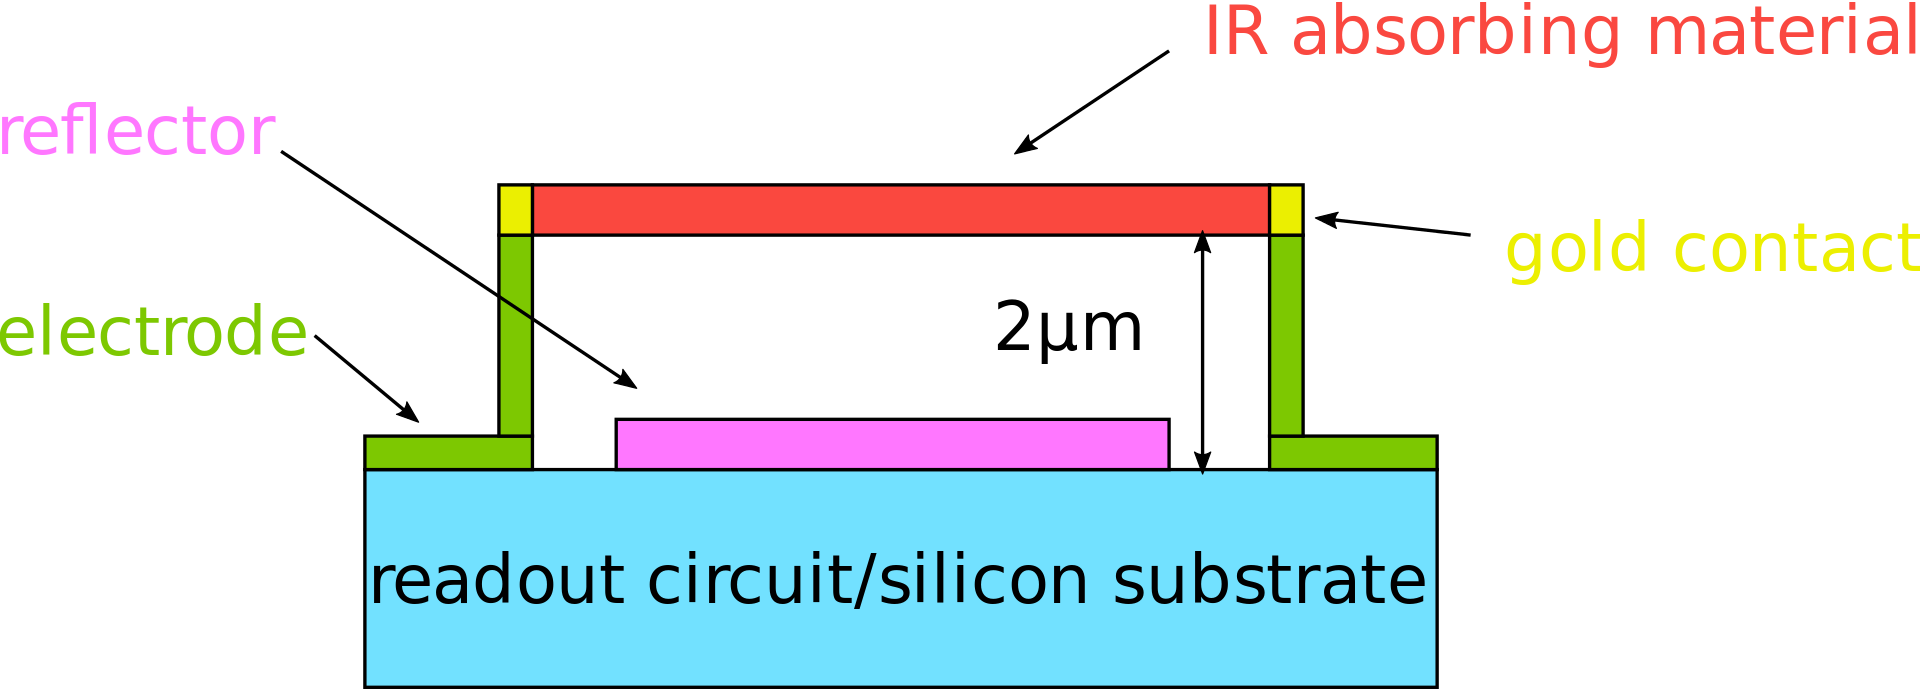
\includegraphics[width=0.4\textwidth]{Images/Temperature/Microbolometer.png}
 \caption{Rapresentation of pixel in a microbolometer detector. When incident radiation arrives on the pixel, temperature increases and electric resistance of the circuit changes, giving rise to a current intensity proportional to radiation intensity.}
\end{figure}


\paragraph{Camera}
We utilize a termographic camera \emph{FLIR A655sc} (\cite{flircamera}) with a spectral range of $\num{7.5}-\SI{14}{\micro\meter}$, resolution $\num{640}\times\num{480}$ and detector pitch \SI{17}{\micro\meter}, equipped with a lens with focal \SI{41.3}{\milli\meter} (field of view \ang{15}).
Temperature evolution is a phenomenon with charateristic time of several seconds, we have a reasonable resolution with frame rate acquisition set at \num{2} FPS.

The temperature conversion between intensity of the radiation and temperature is done by \emph{FLIR} software, setting the appropriate emissivity.

\paragraph{Source}
We use the latest source model, B in chapter \ref{ch:electric}, at different pulse repetition frequencies $f$ and voltage peak values $V_p$. Plasma formation and deposition it's not a continuos phenomenon, it happens in correspondance of voltage pulses, with a charateristic time around \SI{1}{\micro\second}, see chapter \ref{ch:shape}. Given a time interval, $f$ defines the number of pulses that arrives in that interval.

The gas we use to produce plasma is helium, with flow of \SI{2}{\liter/\minute}.

\paragraph{Target}
We use an aluminium target, disk shaped, with radius \SI{7}{\milli\meter} and height \SI{1}{\milli\meter}, on a plastic support with width \SI{5}{\milli\meter}.
Aluminium has specific heat capacity $c_p = \SI{897}{\joule/\kilogram\kelvin}$ and density $\rho = \SI{2700}{\kilogram/\meter^3}$, corresponding to target heat capacity $C = \SI{0.373(5)}{\joule/\kelvin}$.

Target is positioned at a distance of \SI{210}{\milli\meter} from camera lens. At those conditions, once the image is on focus, pixel to pixel distance on acquired frames is \SI{86.4}{\micro\meter}.

We want to study proportionality with distance between target and source, so the target is positioned at a distance of \num{5.5}, \num{7.5} or \SI{9.5}{\milli\meter} from the end of the source head.

\paragraph{Measurements procedure}
Ultimately measurements are done with different voltage pulse repetition frequencies $f$, voltage peak values $V_p$ and distances between target and source $d$.
Once those parameters are set, we follow an approximative timeline:
\begin{itemize}
 \item acquisition of at least \num{4} frames for background evaluation in \SI{2}{\second}
 \item start of gas flow for a minimum of \SI{5}{\second}
 \item start of the discharge for a minimum of \SI{30}{\second}
 \item stop of the discharge and acquisition with only gas flow for \SI{5}{\second}
 \item stop of gas flow
\end{itemize}

Start and end time for those phases can be observed directly from measures.

\section{Temperature profile}
Every frame gives information on the temperature of every pixel of acquired image at a given time, as in figure \ref{fig:exframe}. We are interested in temperature difference, to find them we evaluate background temperature before discharge as the average value acquired before gas opening and subtract it to pixel value in other frames. In a given direction we obtain a graph as in figure \ref{fig:exframe}.
\begin{figure}
 \centering
 \subfloat[Frame $t = \SI{25}{\second}$.]{
    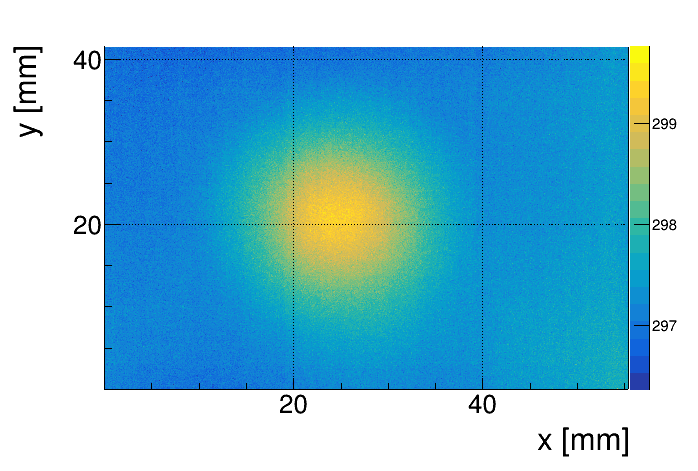
\includegraphics[width=0.48\textwidth]{Images/Temperature/f5t4d4_esframe_25s_2.png}
 }
 \hfill
 \subfloat[$\Delta T$ profile along x direction at $t = \SI{25}{\second}$]{
    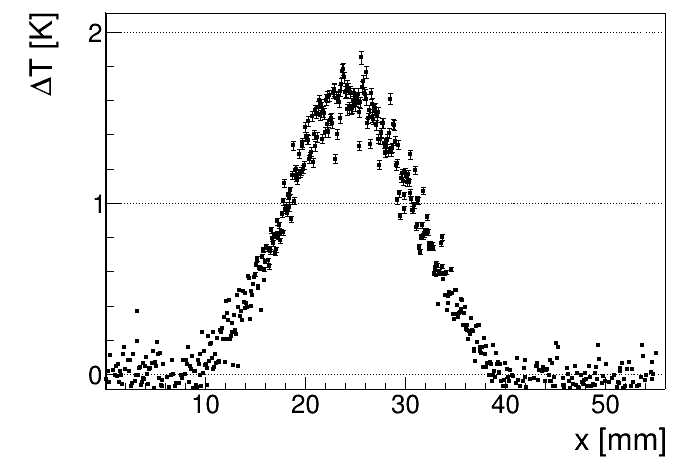
\includegraphics[width=0.48\textwidth]{Images/Temperature/f5t4d4_esprofilo_25s_2.png}
 }
 \caption{Example of measurement during discharge with parameters $f = \SI{5}{\kilo\hertz}$, $V_p = \SI{7.2}{\kilo\volt}$ and $d = \SI{5.5}{\milli\meter}$.}
 \label{fig:exframe}
\end{figure}


Source is pointed to target center, for frames acquired with the discharge we see clearly where the temperature rises and estimate center position. We find the point with maximum temperature and select a square window intersting for temperature evaluation centered on it, with edge \SI{15}{\milli\meter} where it's possible to see the entirety of the target. We find the center position, compatible in each measurements set, at coordinates $x_{c} = \SI{25.06(20)}{\milli\meter}$, $y_{c} = \SI{21.17(20)}{\milli\meter}$.

It's interesting to note that when there is only gas flowing on the target, temperature increases radially from the center, in an area larger then the target area, while when there is plasma, temperature increases rapidly in an area compatible with the target dimensions. It's possible that gas before ionization creates a gas layer with a radius larger then the target radius, but if we observe temperature increase only around the target it doesn't gives problems in heat power evaluation due to discharge.

From each of those frames we evaluate the average temperature difference and it's evolution, as shown in figure \ref{fig:Tavg}. This graph allows to extrapolate time intervals for gas flow and discharge: where temperature changes rapidly we have gas opening, source activation, discharge end and gas flow stop. In figure \ref{fig:dis_profiles} an example of how temperature profile changes during discharge.
\begin{figure}
 \centering
 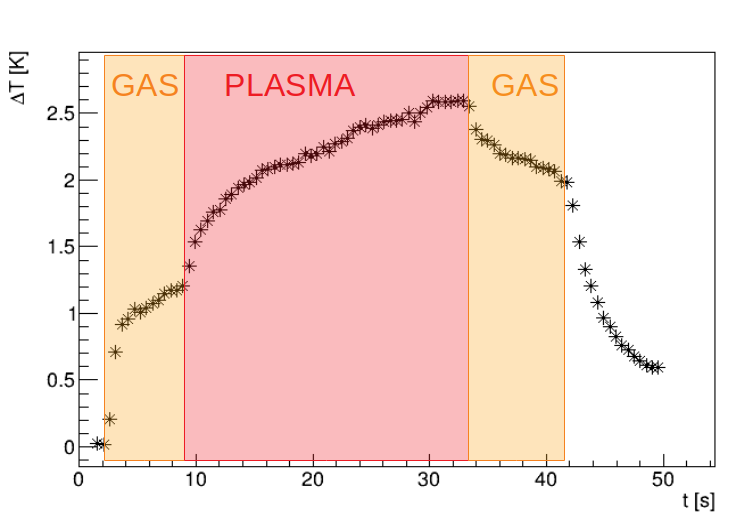
\includegraphics[width=0.6\textwidth]{Images/Temperature/f5t4d4_Tavg_lines.png}
 \caption{Average increase in temperature for every frame at different times, on a square around the target. There are three phases highlighted: gas phase before source activation, plasma phase and gas phase after source power off.}
 \label{fig:Tavg}
\end{figure}

\begin{figure}
 \centering
 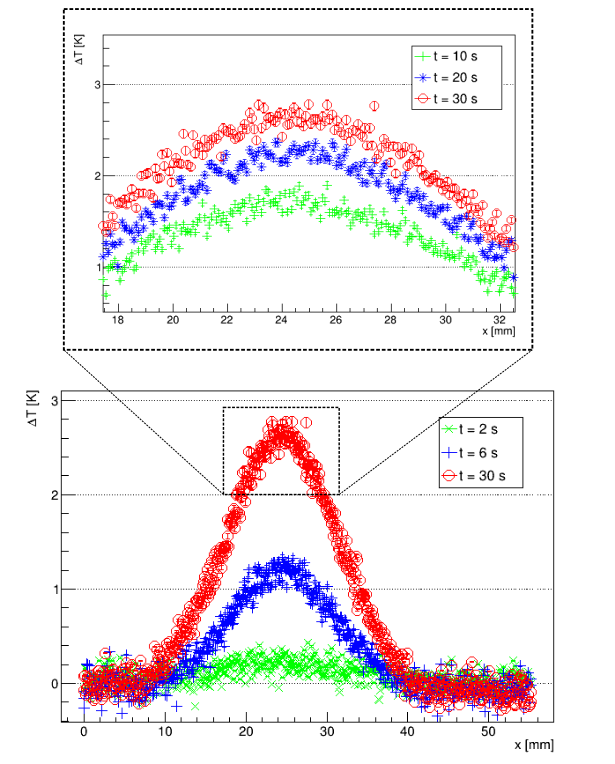
\includegraphics[width=0.6\textwidth]{Images/Temperature/f5t4d4_profilo_tempi_zoom.png}
 \caption{Evolution of temperature profile in x direction, with a zoom on the region around the target, for different times and phases: $t = \SI{2}{\second}$ before gas opening, $t = \SI{6}{\second}$ after gas opening and before discharge, $t = $\num{10}, \num{20}, \SI{30}{\second} during discharge. }
 \label{fig:dis_profiles}
\end{figure}



\section{Power estimation}
During the plasma phase, temperature increase in target can be defined as the sum of power deposition plus thermalization contributions (see \cite{Pimazzoni2018}), as in equation \ref{eq:dT}, where $m$ is the mass of the portion of target considered, $c_p$ is aluminium specific heat capacity, $P$ is power deposited by plasma on target, $T_{0}$ is a temperature limit and $k$ a costant parameter dependant from the target.
\begin{equation}
 m c_p \frac{dT}{dt} = P - k(T-T_{\text{lim}})
 \label{eq:dT}
\end{equation}

The anlytical result of this equation is an exponential function, as in figure \ref{fig:dTfit} for the center pixel in the image. The downside of the exponential fit it's that isn't possible to evaluate the contribution of power deposition from it. If we consider temperature variation only for temperatures close to $T_{0}$, where the thermalization contribute is neglectable, we can extrapolate parameter $P$ with a linear fit. The power parameter that we evaluate this way it's not a precise value because there are also thermalization contributes, but we can use it to study the behavior varying other parameters.
\begin{figure}
 \centering
 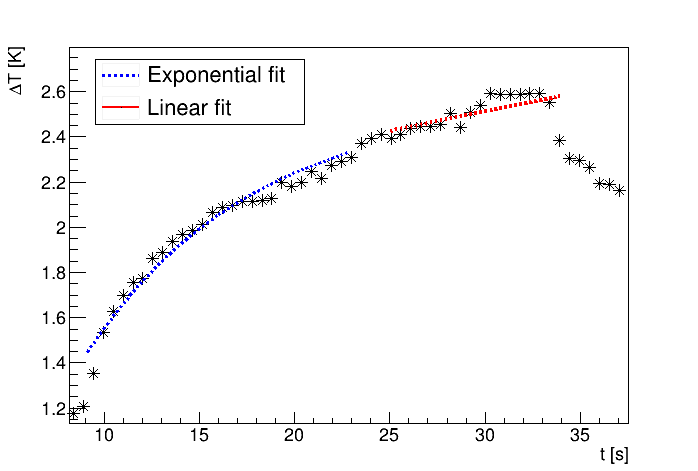
\includegraphics[width=0.6\textwidth]{Images/Temperature/f5t4d4_fits.png}
 \caption{Average increase of temperature. The exponential fit shows the analytical solution for equation \ref{eq:dT}, the linear fit is how power is extrapolated.}
 \label{fig:dTfit}
\end{figure}

To assure that we are observing temperature variation only inside the target, we consider every pixel in a radius of \SI{7}{\milli\meter} from the center of plasma application. The mean temperaure variation in those conditions follows equation \ref{eq:dTpix}, where $\rho$ is aluminium density, $h$ is target width, $A_p$ is target area, $T_{\text{avg}}$ is the average temperature of a pixel, $T_p$ is the temperature of a pixel.
\begin{equation}
 m c_{p} T_{\text{avg}}(t) = \rho h A_{p}\frac{\sum_{\text{pixels}} T_{p}}{N_{\text{pixels}}} = P t + T_{0}
 \label{eq:dTpix}
\end{equation}


Plasma deposition isn't continuos in time but it happens within time intervals, as we can see in chapter \ref{ch:shape}.
Power evaluated considering the total time interval of plasma application is an effective power $P_{\text{eff}}$ that doesn't take into consideration the real time interval of interaction between plasma and target, a fraction of the total one. We can estimate the power associated with a single pulse $P_{\text{pulse}}$, considering the time interval for the interaction of every pulse $\Delta t_{\text{pulse}}$ multiplied by the rate of pulses during the discharge $f$, as in equation \ref{eq:power}. An appropriate time pulse duration is $\Delta t_{\text{pulse}} = \SI{1}{\micro\second}$, as in chapter \ref{ch:shape}.
\begin{equation}
 P_{\text{pulse}} = \frac{P_{\text{eff}}}{\Delta t_{\text{pulse}} \, f}
 \label{eq:power}
\end{equation}


\paragraph{Pulse rate dependency}
We extrapolate power parameter with different pulse repetition rate, voltage peak value set at $V_{p} = \SI{7.2}{\kilo\volt}$ and distance between source and target $d = \SI{5.5}{\milli\meter}$. In figure \ref{fig:Pfr} there are effective power during the discharge and the pulse power relative to a single pulse. As expected the effective power is proportional to frequency of pulses: greater frequency means more pulses in a given time. It's instead intersting to note that power for a single pulse decreases with increasing pulse rate. 
An explanation could be that for different pulse repetition rate the time interval relative to the single pulse, i.e. the time interval during which we see plasma bullets, decreases from $\Delta t_{\text{pulse}} = \SI{1}{\micro\second}$ for $f = \SI{5}{\kilo\hertz}$ to values around $\Delta t_{\text{pulse}} = \SI{500}{\nano\second}$ for $f = \SI{25}{\kilo\hertz}$. This result could imply that for higher frequencies we have bullets more rapid.
\begin{figure}
 \centering
 \subfloat[Average power during discharge.]{
    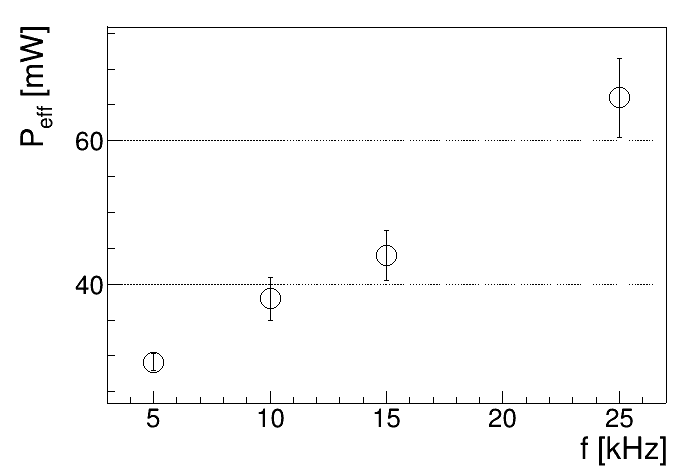
\includegraphics[width=0.48\textwidth]{Images/Temperature/Peff_fr_2.png}
 }
 \subfloat[Power relative to a single voltage pulse.]{
    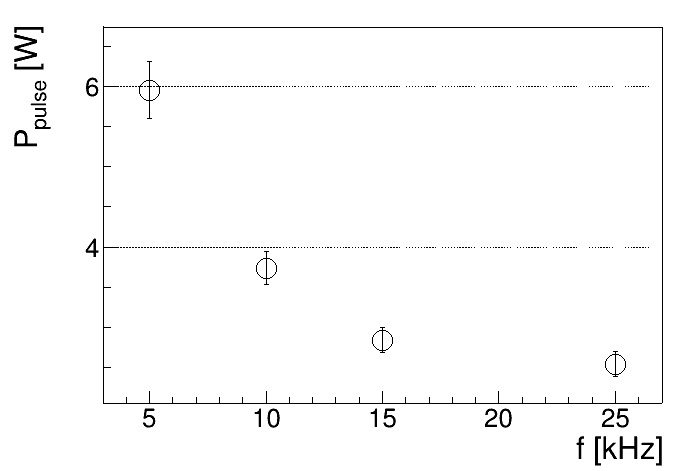
\includegraphics[width=0.48\textwidth]{Images/Temperature/Ppulse_fr_2.png}
 }
 \caption{Plasma power deposition on target for different pulse repetition rates.}
 \label{fig:Pfr}
\end{figure}


\paragraph{Voltage peak value dependency}
We measure how temperature increases with distance between source and target $d = \SI{5.5}{\milli\meter}$ and pulse repetition rate $f = \SI{5}{\kilo\hertz}$, for different voltage values. In figure \ref{fig:PVp} we can see that power for the single pulse is correlated with the voltage peak value and increases rapidly when voltage increases. This behavior is expected because with an higher peak voltage value there is more electrical power transfered from the source and we have higher bullet velocity, as seen in chapter \ref{ch:shape}.
\begin{figure}
 \centering
 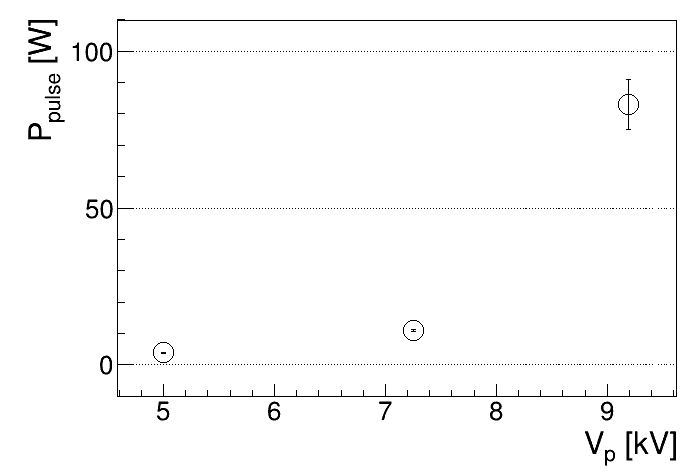
\includegraphics[width=0.6\textwidth]{Images/Temperature/Ppulse_Vp_2.png}
 \caption{Plasma power of a single pulse for different voltage peak values.}
 \label{fig:PVp}
\end{figure}

\paragraph{Distance dependency}
We measure influence of the distance between target and source, setting voltage peak at $V_{p} = \SI{7.2}{\kilo\volt}$ and $f = \SI{5}{\kilo\hertz}$. In figure \ref{fig:Pd} we can see how power decreases with incresing distance, as expected because for higher distances between source and target, bullets lose more energy before the impact and will transfer less energy to the target. For distance going from \SI{5.5}{\milli\meter} to \SI{7.5}{\milli\meter} we can find a pulse power loss rate of \SI{0.28(5)}{\watt/\milli\meter}.
\begin{figure}
 \centering
 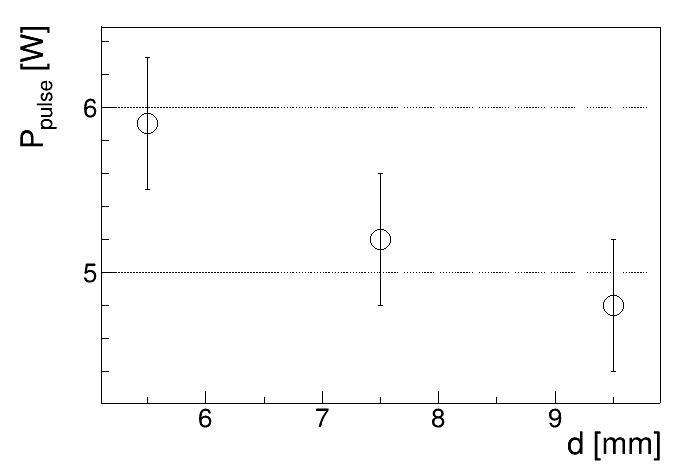
\includegraphics[width=0.6\textwidth]{Images/Temperature/Ppulse_d_2.png}
 \caption{Plasma power of a single pulse for different target distances.}
 \label{fig:Pd}
\end{figure}
